\documentclass[16pt, a4paper, two column]{article}
\usepackage[utf8]{inputenc}
\usepackage[a4paper, total={6in, 8in}, margin = 1in]{geometry}
\usepackage{graphicx}
\graphicspath{{figs/}}
\usepackage{amsmath}
\usepackage{amssymb}
\usepackage{array}
\usepackage{listings}
%\usepackage{iithtlc}
\usepackage{tikz}
\usetikzlibrary{shapes,arrows}
\usepackage{txfonts}
\usepackage{stfloats}
%\usepackage{supcaption}
\def\inputGnumericTable{}
\usepackage[latin1]{inputenc}                                 %%
    \usepackage{color}                                            %%
    \usepackage{array}                                            %%
    \usepackage{longtable}                                        %%
    \usepackage{calc}                                             %%
    \usepackage{multirow}                                         %%
    \usepackage{hhline}                                           %%
    \usepackage{ifthen}
\providecommand{\brak}[1]{\ensuremath{\left(#1\right)}}
\providecommand{\pr}[1]{\ensuremath{\Pr\left(#1\right)}}
\usepackage{url}
\def\UrlBreaks{\do\/\do-}
\lstset{
%language=C,
frame=single, 
breaklines=true,
columns=fullflexible
}

\title{Random Numbers Assignmnet}
\author{Hema Sri Cheekatla, CS21BTECH11013}
\begin{document}
\maketitle
\section*{Question 1.1}Generate $10^6$ samples of U using a C program and save into a file called uni.dat.
\section*{Solution:}
Download the following files and execte the C program.
\begin{lstlisting}
wget https://github.com/Hema-Sri-Ch/AI1110-Assignments/Assignment/codes/exrand.c
wget https://github.com/Hema-Sri-Ch/AI1110-Assignments/Assignment/codes/coeffs.h
\end{lstlisting}
And run the following commands in the terminal to execute the C program files
\begin{lstlisting}
gcc -o out exrand.c coeffs.h -lm
./out
\end{lstlisting}
Then the corresponding "uni.dat" file will be created with $10^6$ samples of U.

\section*{Question1.2}
Load the uni.dat file into python and plot the emprical CDF of U using the samples in uni.dat. The CDF is defined as 
\begin{align}
	F_U(x) = \pr{U \leq x}
\end{align}
\section*{Solution}
The following code plots Fig. \ref{fig:uni_cdf} in the figs folder(Comment out or remove comments for some lines accordingly)
\begin{lstlisting}
wget https://github.com/Hema-Sri-Ch/AI1110-Assignments/Assignment/codes/cdf_plot.py
\end{lstlisting}
And execute the following command in the terminal 
\begin{lstlisting}
python3 cdf_plot.py
\end{lstlisting}
\begin{figure}[h]
	\centering
	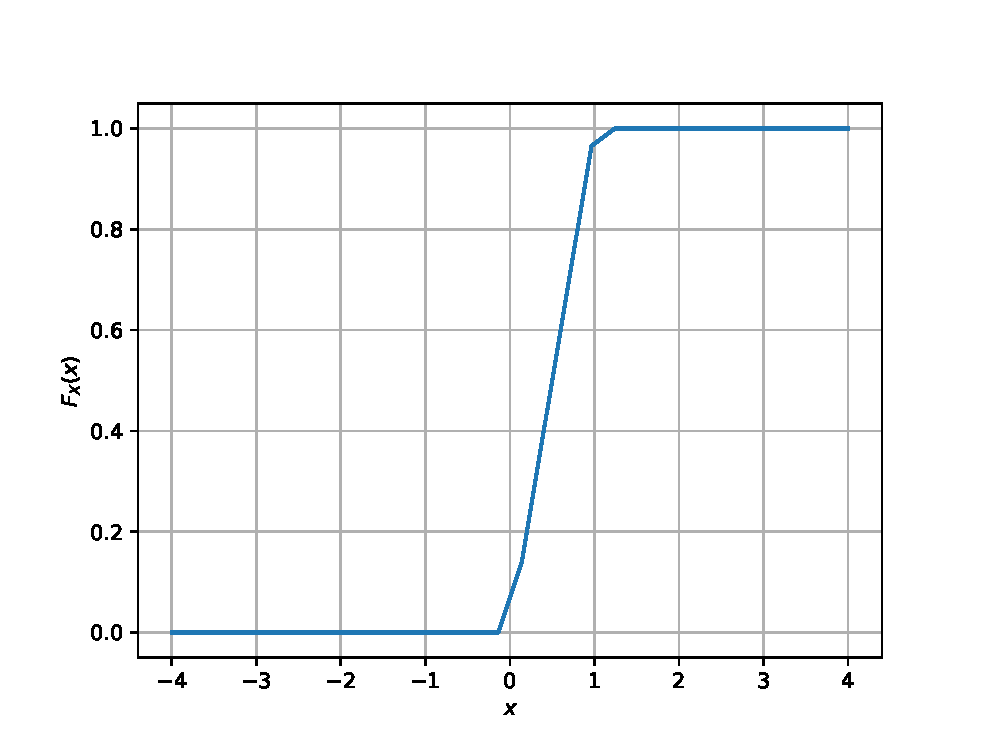
\includegraphics[width=\columnwidth]{uni_cdf}
	\caption{The CDF of $U$}
	\label{fig:uni_cdf}
\end{figure}
\section*{Question 1.3} Find a theoretical expression for $F_U(x)$.

\section*{Solution}
We know that the PDF of a uniform distribution function in a particular intervel (a, b) is given by,
\begin{align}
	f(x) &= \begin{cases} \frac{1}{b-a} &,\text{ for } a \leq x \leq b \\
	0 &, otherwise\end{cases}
\end{align}

Hence, the CDF of a uniform distribution function is given as follows in a particular interval (a, b)

\begin{align}
	F_U(x) &= \begin{cases} 0 &, \text{ for } x < a\\
	 \frac{x-a}{b-a} &, \text{ for } a \leq x \leq b \\
	 1 &, \text{ for } x > b\end{cases}
\end{align}

In Our case, the intervel is (0, 1). Hence the theoretical expression for $F_U(x)$ is given as follows,

\begin{align}
	F_U(x) &= \begin{cases} 0 &, \text{ for } x < 0\\
	 x &, \text{ for } 0 \leq x \leq 1 \\
	 1 &, \text{ for } x > 1\end{cases}
\end{align}

\section*{Question 1.4}
The mean of $U$ is defined as 
\begin{align}
	E[U] &= \frac{1}{N}\sum_{i=1}^{N} U_i
\end{align}
and its variance as 
\begin{align}
	\text{var}[U] &= E[U-E[U]]^2
\end{align}
Write a C program to find the mean and the variance of $U$
\section*{Solution}
Download the following files and execte the C program.
\begin{lstlisting}
wget https://github.com/Hema-Sri-Ch/AI1110-Assignments/Assignment/codes/exrand.c
wget https://github.com/Hema-Sri-Ch/AI1110-Assignments/Assignment/codes/coeffs.h
\end{lstlisting}
And run the following commands in the terminal to execute the C program files
\begin{lstlisting}
gcc -o out exrand.c coeffs.h -lm
./out
\end{lstlisting}
The Mean and Variance of $U$ is written as output in the terminal.
\section*{Question 1.5}
Verify your result theoretically given that
\begin{align}
	E[U^k] &= \int_{-\infty}^{\infty}x^k dF_U(x)
\end{align}
\section*{Solution}
If k = 1, then E[$U^1$] is nothing but the mean of this uniform distribution,\newline
Theoretically, we have 
\begin{align}
	F_U(x) &= \begin{cases} 0 &, \text{ for } x < 0\\
	 x &, \text{ for } 0 \leq x \leq 1 \\
	 1 &, \text{ for } x > 1\end{cases}
\end{align}
Hence $dF_U(x)$ can be written as follows,
\begin{align}
	dF_U(x) &= f(x) = \begin{cases} 1 &,\text{ for } 0 \leq x \leq 1 \\
	0 &, otherwise\end{cases} \\
	\implies E[U] &= \int_{0}^{1} x \,dx \\
	&= 0.5
\end{align}
Hence our theoretical mean is 0.5, where as we got our practical mean as 0.500007, which is almost same.\newline
Hence our expression is verified for k = 1.\newline
Similarly we can consider k = 2, then we get,
\begin{align}
	E[U^2] &= \int_{0}^{1} x^2 \, dx \\
	&= 0.333333 
\end{align}
Hence our theoretical value of $E[U^2]$ is 0.333333, where we got our practical value of $E[U^2]$ as 0.333308, which is again almost same as that of theoretical value.\newline
Hence Verified.

\section*{Question 2.1}
Generate $10^6$ samples of the random variable
\begin{align}
	X &= \sum_{i=1}^{12} U_i - 6
\end{align}
usign a C program, where $U_i, i = 1, 2, ..., 12$ are a set of independent uniform random variables between 0 and 1 and save in a file called gau.dat
\section*{Solution}
Download the following files and execte the C program.
\begin{lstlisting}
wget https://github.com/Hema-Sri-Ch/AI1110-Assignments/Assignment/codes/exrand.c
wget https://github.com/Hema-Sri-Ch/AI1110-Assignments/Assignment/codes/coeffs.h
\end{lstlisting}
And run the following commands in the terminal to execute the C program files
\begin{lstlisting}
gcc -o out exrand.c coeffs.h -lm
./out
\end{lstlisting}
Then the corresponding "gau.dat" file will be created with $10^6$ samples of X.
\section*{Question 2.2}
Load gau.dat in python and plot the emprical CDF of X using the samples in gau.dat. What properties does a CDF have?
\section*{Solution}
The following code plots Fig. \ref{fig:gauss_cdf} in the figs folder(Comment out or remove comments for some lines accordingly)
\begin{lstlisting}
wget https://github.com/Hema-Sri-Ch/AI1110-Assignments/Assignment/codes/cdf_plot.py
\end{lstlisting}
And execute the following command in the terminal 
\begin{lstlisting}
python3 cdf_plot.py
\end{lstlisting}
\begin{figure}[h]
	\centering
	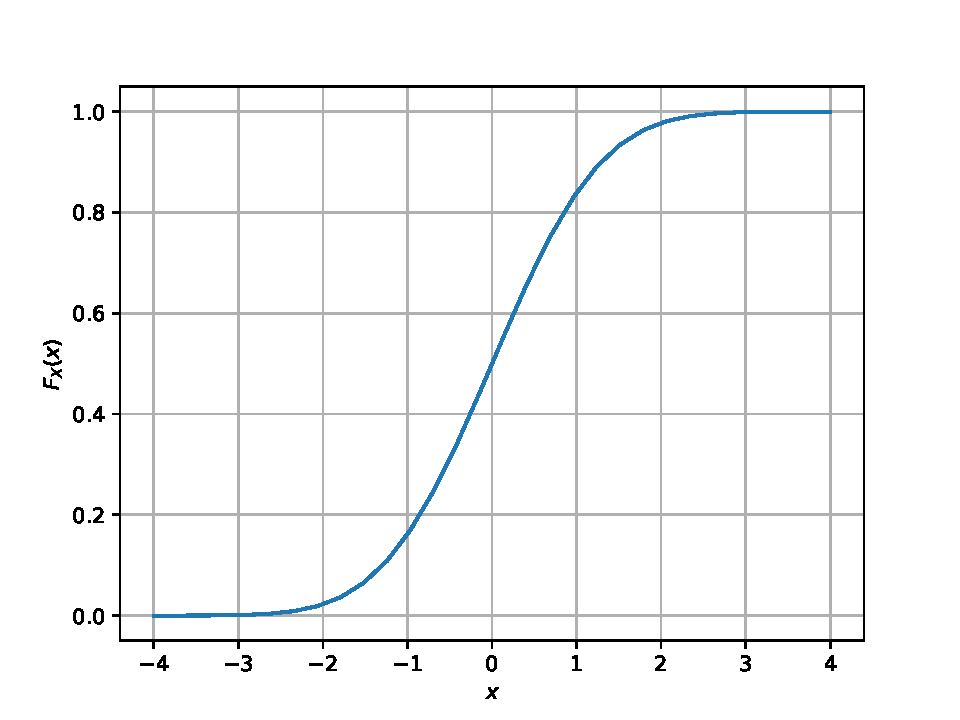
\includegraphics[width=\columnwidth]{gauss_cdf}
	\caption{The CDF of $X$}
	\label{fig:gauss_cdf}
\end{figure}

\section*{Question 2.3}
Load gau.dat in python and plot the empirical PDF of $X$ using the samples in gau.dat. The PDF of $X$ is defined as
\begin{align}
p_{X}(x) = \frac{d}{dx}F_{X}(x)
\end{align}
What properties does the PDF have?
\section*{Solution}
The following code plots Fig. \ref{fig:gauss_pdf} in the figs folder(Comment out or remove comments for some lines accordingly)
\begin{lstlisting}
wget https://github.com/Hema-Sri-Ch/AI1110-Assignments/Assignment/codes/pdf_plot.py
\end{lstlisting}
And execute the following command in the terminal 
\begin{lstlisting}
python3 pdf_plot.py
\end{lstlisting}
\begin{figure}[h]
	\centering
	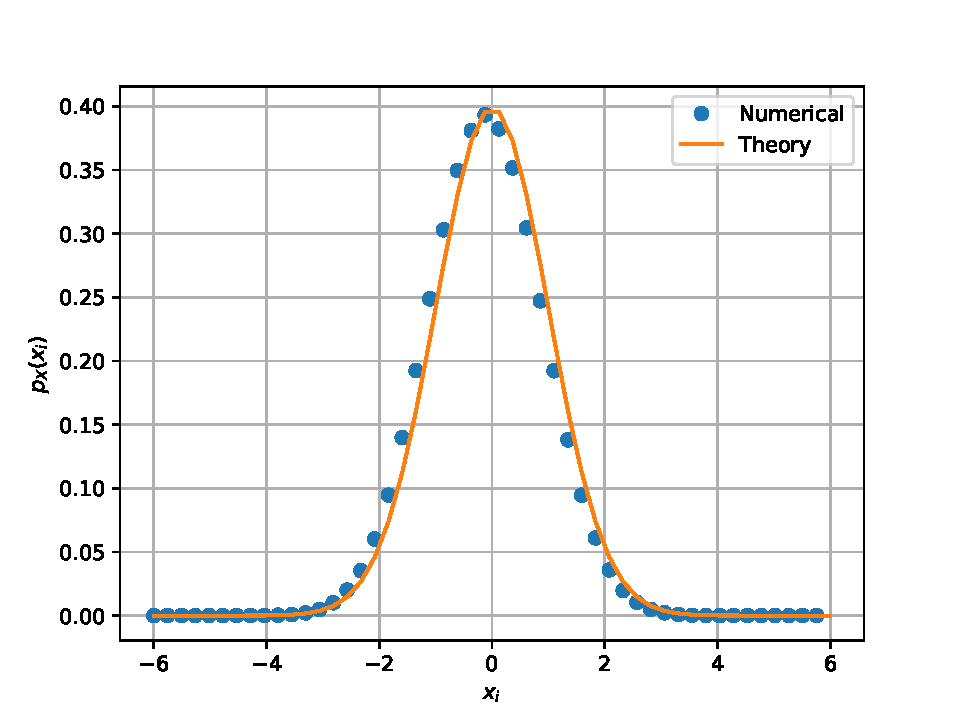
\includegraphics[width=\columnwidth]{gauss_pdf}
	\caption{The PDF of $X$}
	\label{fig:gauss_pdf}
\end{figure}

\section*{Question 2.4}
Find the mean and variance of $X$ by writing a C program
\section*{Solution}
Download the following files and execte the C program.
\begin{lstlisting}
wget https://github.com/Hema-Sri-Ch/AI1110-Assignments/Assignment/codes/exrand.c
wget https://github.com/Hema-Sri-Ch/AI1110-Assignments/Assignment/codes/coeffs.h
\end{lstlisting}
And run the following commands in the terminal to execute the C program files
\begin{lstlisting}
gcc -o out exrand.c coeffs.h -lm
./out
\end{lstlisting}
The Mean and Variance of $X$ is written as output in the terminal.
\section*{Question 2.5}
Given that,
\begin{align}
	p_X(x) &= \frac{1}{\sqrt{2\pi}}exp(-\frac{x^2}{2}) &, -\infty < x < \infty
\end{align}
Find the mean and variance of this Gaussian distribution theoretically
\section*{Solution}
We know that,
\begin{align}
	Mean &= E[U] = \int_{-\infty}^{\infty} x p_X(x) \, dx\\
	&= \int_{-\infty}^{\infty} x \frac{1}{\sqrt{2\pi}}exp(-\frac{x^2}{2}) \, dx
\end{align}
Since the function $x \frac{1}{\sqrt{2\pi}}exp(-\frac{x^2}{2})$ is an odd function, its integral in the interval $(-\infty, \infty)$ is zero.
Hence the Theoretical Mean is 0, whereas the practical Mean we have obtained is 0.000326 which is almost as same as that of Theoretical Mean\newline

We know that,
\begin{align}
	Varience &= E[U^2] - E[U]^2 \\
	\implies Variance &= E[U^2] \\
	Variance &= E[U^2] = \int_{-\infty}^{\infty} x^2 p_X(x) \, dx \\
	&= \int_{-\infty}^{\infty} x^2 \frac{1}{\sqrt{2\pi}}e^{-\frac{x^2}{2}} \,dx \\
	&= \frac{2\sqrt{2} }{\sqrt{2\pi}} \int_{-\infty}^{\infty} x^2 e^{-x^2} \, dx \\
	\text{ since, } \int_{-\infty}^{\infty} x^2 e^{-x^2} \, dx &= \frac{\sqrt{\pi}}{2} \\
	\implies Variance &= 1
\end{align}
Hence the Theoretical Variance is 1, whereas the practical Varaince we have obtained is 1.000907 which is almost as same as that of the Theoretical Varaince\newline
\section*{Question 3.1}
Generate samples of 
\begin{align}
V = -2\ln\brak{1-U}
\end{align}
and plot its CDF.
\section*{Solution}
Download the following files and execte the C program.
\begin{lstlisting}
wget https://github.com/Hema-Sri-Ch/AI1110-Assignments/Assignment/codes/exrand.c
wget https://github.com/Hema-Sri-Ch/AI1110-Assignments/Assignment/codes/coeffs.h
\end{lstlisting}
And run the following commands in the terminal to execute the C program files
\begin{lstlisting}
gcc -o out exrand.c coeffs.h -lm
./out
\end{lstlisting}
Then the corresponding "req.dat" file will be created with $10^6$ samples of V.
The following code plots Fig. \ref{fig:req_cdf} in the figs folder.(Comment out or remove comments for some lines accordingly)
\begin{lstlisting}
wget https://github.com/Hema-Sri-Ch/AI1110-Assignments/Assignment/codes/cdf_plot.py
\end{lstlisting}
And execute the following command in the terminal 
\begin{lstlisting}
python3 cdf_plot.py
\end{lstlisting}
\begin{figure}[h]
	\centering
	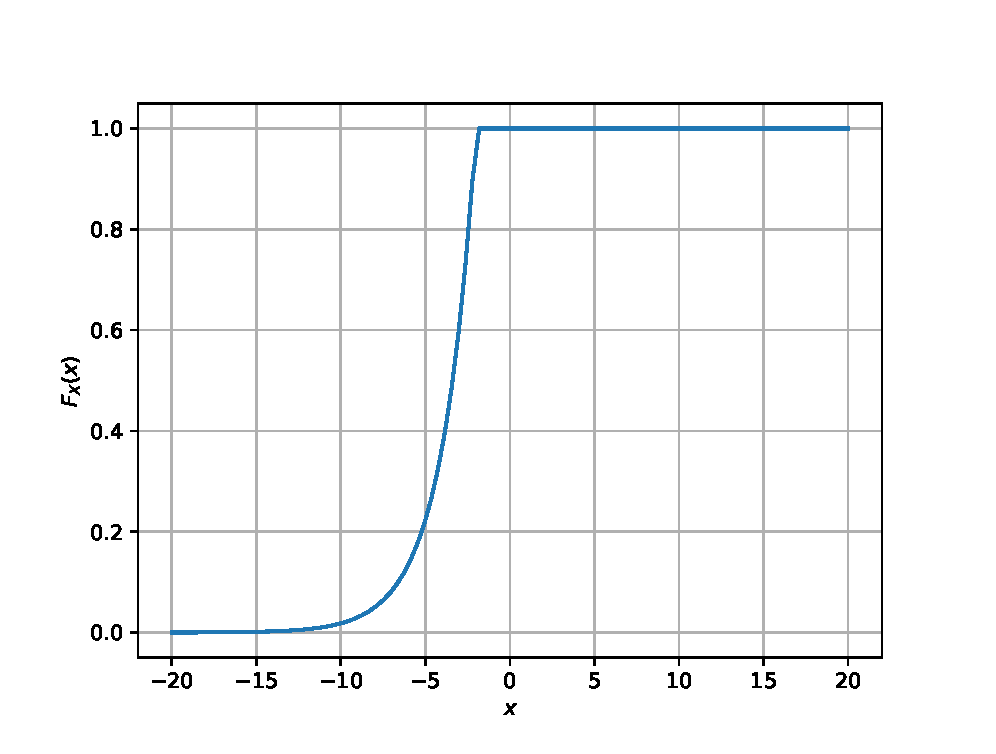
\includegraphics[width=\columnwidth]{req_cdf}
	\caption{The CDF of $V$}
	\label{fig:req_cdf}
\end{figure}
\section*{Question 3.2}
\begin{align}
	V &= -2 \ln(1-U)
\end{align}
Find a theoretical expression for $F_V(x)$.
\section*{Solution}
We know that,

\begin{align}
	F_V(x) &= P(V \leq x) \\
	F_V(x) &= P(-2 \ln(1-U) \leq x) \\
	F_V(x) &= P(\ln(1-U) \geq -\frac{x}{2}) \\
	F_V(x) &= P(1-U \geq e^{-\frac{x}{2}}) \\
	F_V(x) &= P(U \leq 1-e^{-\frac{x}{2}}) \\
	F_V(x) &= F_U(1-e^{-\frac{x}{2}}) \\
	\text{Hence, } F_V(x) &= \begin{cases} 0 &, x < a \\
	1-e^{-\frac{x}{2}} &, a \leq x \leq b \\
	1 &, x > b \end{cases}
\end{align}
\end{document}
